


\chapter{Fake background}

The misidentified lepton backgrounds are estimated with full data driven method from the collision data. In $\Hmuhad$ channel,  the misidentification $\tau$ lepton rate is obtained from independent Z + jets data sets and then apply the rate to an control region that orthogonal to the signal region to estimate the misidentified lepton backgrounds. This control region is referred as the misidentified lepton estimation region. 

Two set of Z + jets data sets are used, $Z\rightarrow\mu\mu$ and $Z\rightarrow e e$, to estimate the misidentified lepton rate in order to increase the statistics in the estimation.  In both cases, Z bosons are selected in the invariant mass window $70<M_{ll}<110$ GeV. In $Z\rightarrow\mu\mu$, the trigger HLT\_IsoMu24 or HLT\_IsoTkMu24 is used. Both muons are required to have $\pt>26$GeV, $|\eta|<2.4$, cut based tight muon isolation($I^{\mu}_{rel}<0.15$) and passing the muon medium ID. In the $Z\rightarrow e e$ case, the trigger HLT\_singleE25eta2p1Tight is used. Both electrons are required to pass $\pt>26$ GeV, $|\eta|<2.1$, cut based tight electron isolation($I^{e}_{rel}<0.1$) and passing MVANonTrigWP80 ID. In the Z+jets samples, with the selected Z boson in an event, the remaining jets are checked if they pass $\tau$ ID. The misidentified $\tau$ lepton ratio $\tau(f_{\tau})$ is calculated as in Equation .~\ref{eq:1}, together with one related ratio $f_{\tau}$.

\begin{align} 
\tau(f_{\tau})&=\frac{f_{\tau}}{1-f_{\tau}} \label{eq:1}\\
f_{\tau}&=\frac{N_{\tau}(Z+jets\ tau\ tight\ Iso)}{N_{\tau}(Z+jets\ tau\ very\ loose\ Iso)} \label{eq:2}
\end{align}

$f_{\tau}$ is the ratio between number of jets that pass tight $\tau$ MVA isolation ID and number of jets that pass very loose $\tau$ MVA isolation ID. The contribution from Diboson sample are subtracted with simulation, in which the third leptons are genuine leptons. In the events, besides the genuine leptons, jets that pass $\tau$ identification are also required to have $\pt>30$ GeV and $|\eta|<2.3$. With the ratio $f_{\tau}$ , misidentified rate $\tau(f_{\tau})$(Equation.~\ref{eq:2}) is applied as a weight to the misidentified lepton estimation control region, which is defined in the same criteria as the signal region, besides $\tau$ leptons are required to pass very loose isolation and not pass the tight isolation. The misidentified $\tau$ lepton rate $\tau(f_{\tau})$ shows dependence on tau $\pt$ and tau decay mode, thus $\tau(f_{\tau})$ is applied in term of tau $\pt$ and tau decay modes. The distribution of $f_{\tau}$ is shown in Fig.~ \ref{fig:fakerationumber}, which shows a comparison of the estimated $f_{\tau}$ between data and simulated Z+jets samples. 

\begin{figure}[htbp] 
     \centering
     \subfigure[tau decay mode 0]{ 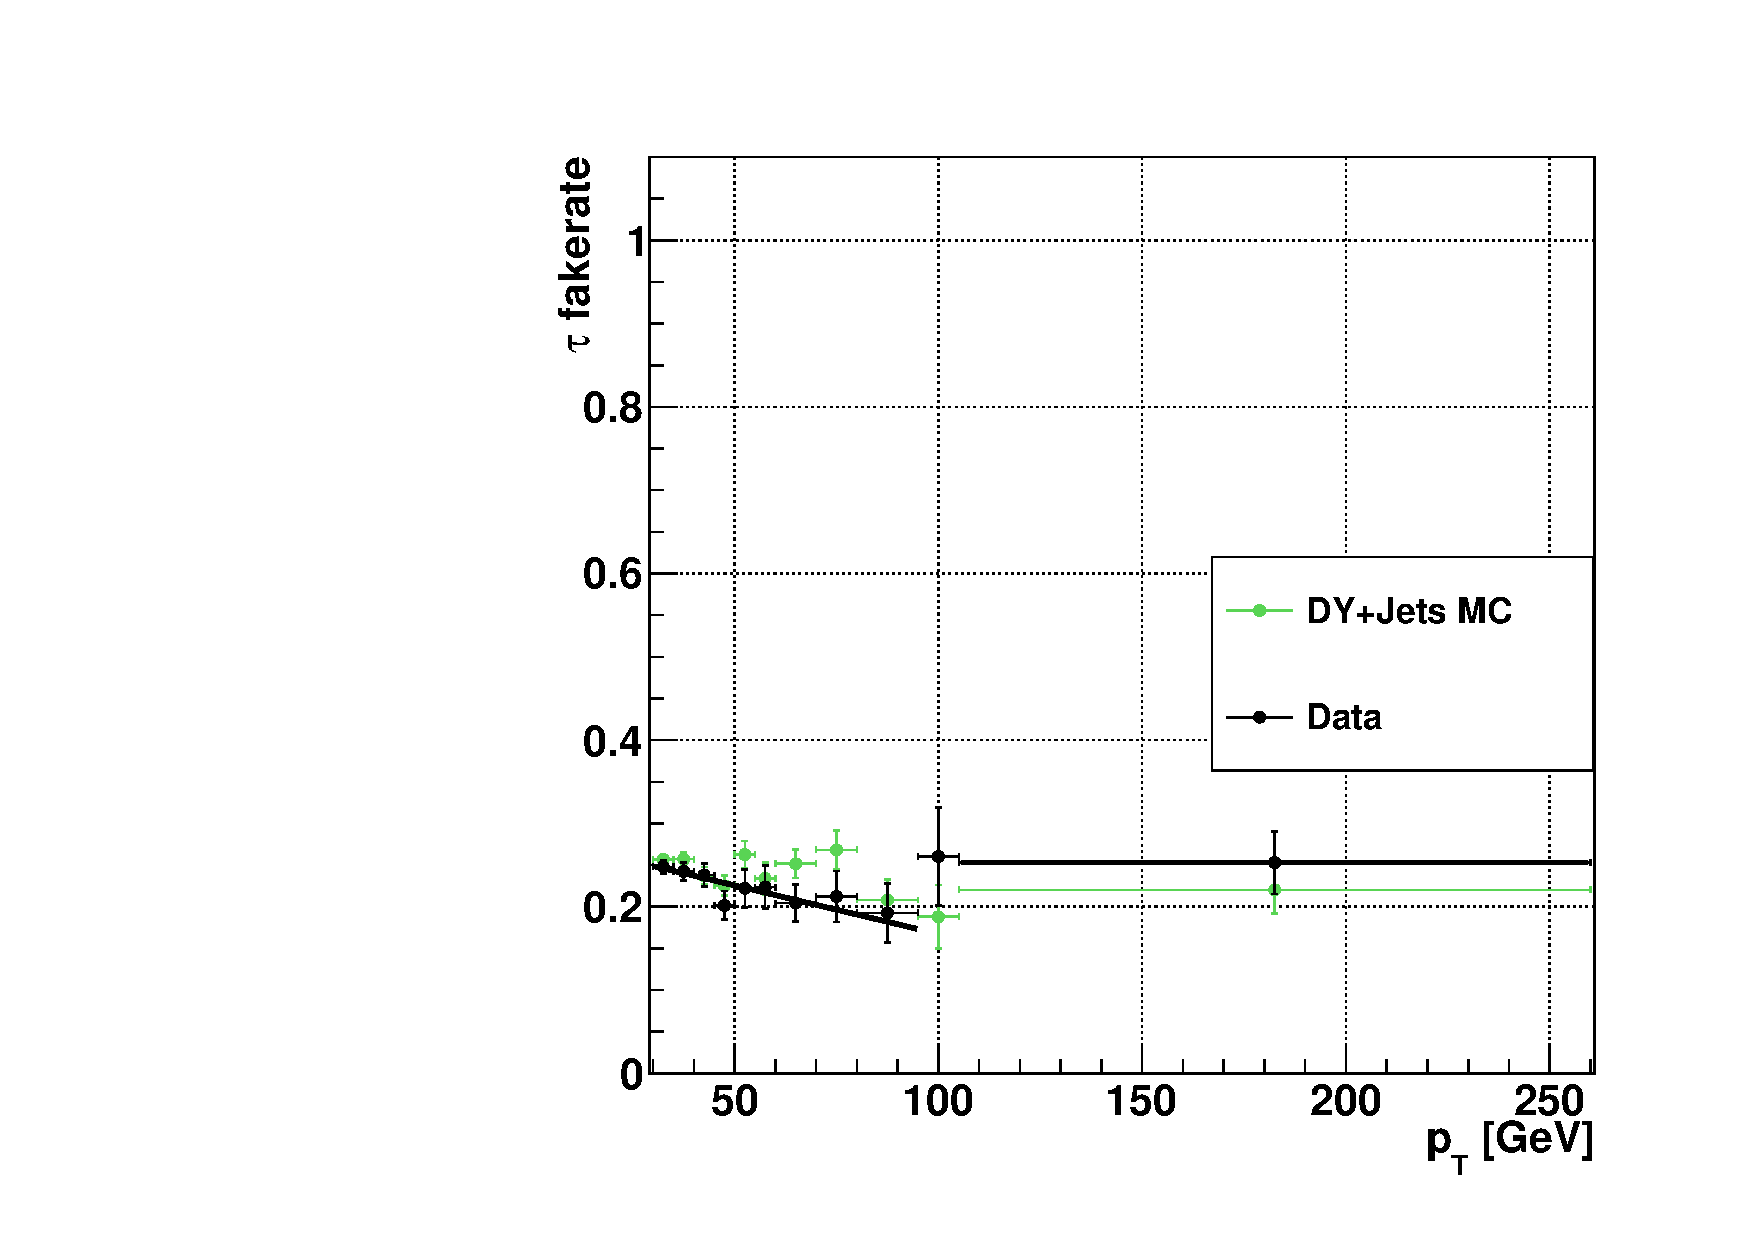
\includegraphics[width=0.3\textwidth]{chapterfakerate/preselectionDecay0_preselectionVLooseIsoDecay0_tPt_fakeRate.pdf}}
     \subfigure[tau decay mode 1]{ 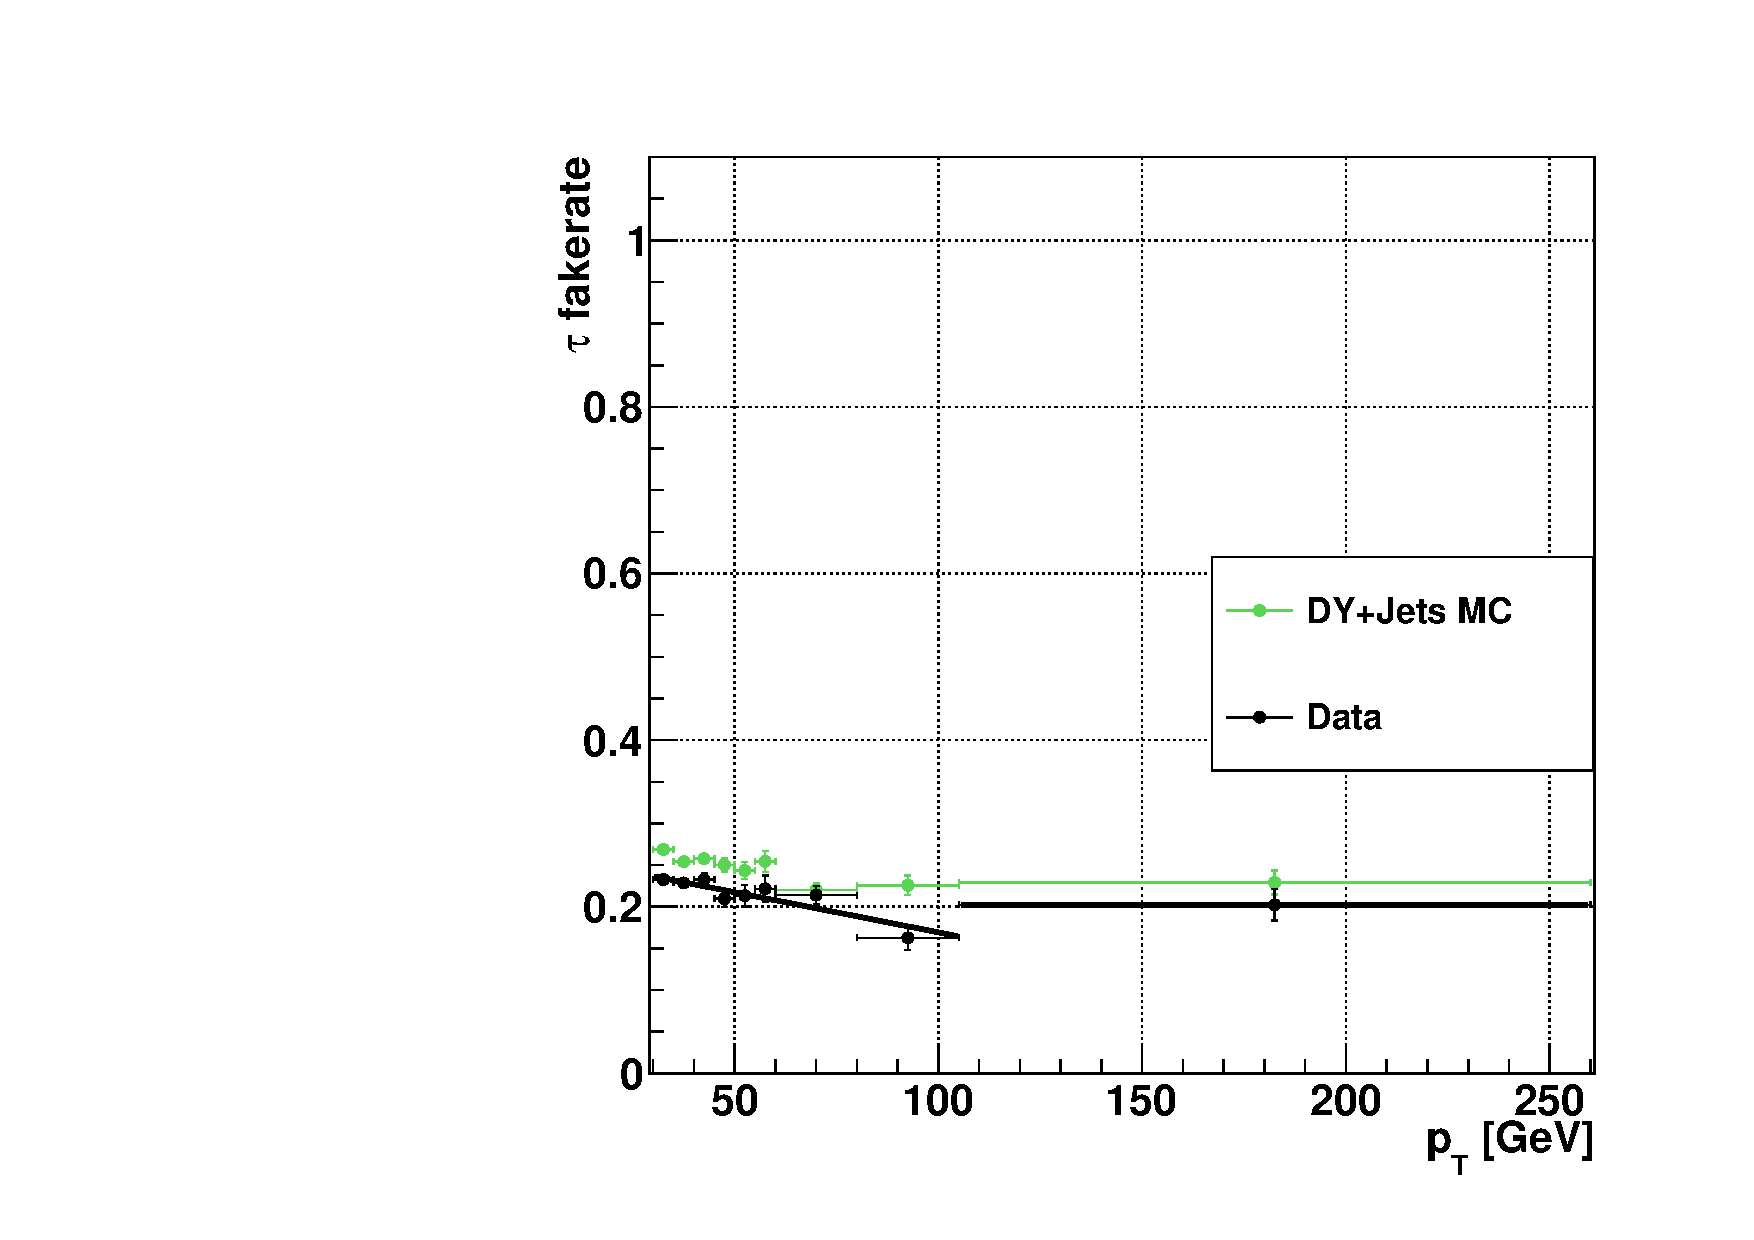
\includegraphics[width=0.3\textwidth]{chapterfakerate/preselectionDecay1_preselectionVLooseIsoDecay1_tPt_fakeRate.pdf}}
      \subfigure[tau decay mode 10]{ 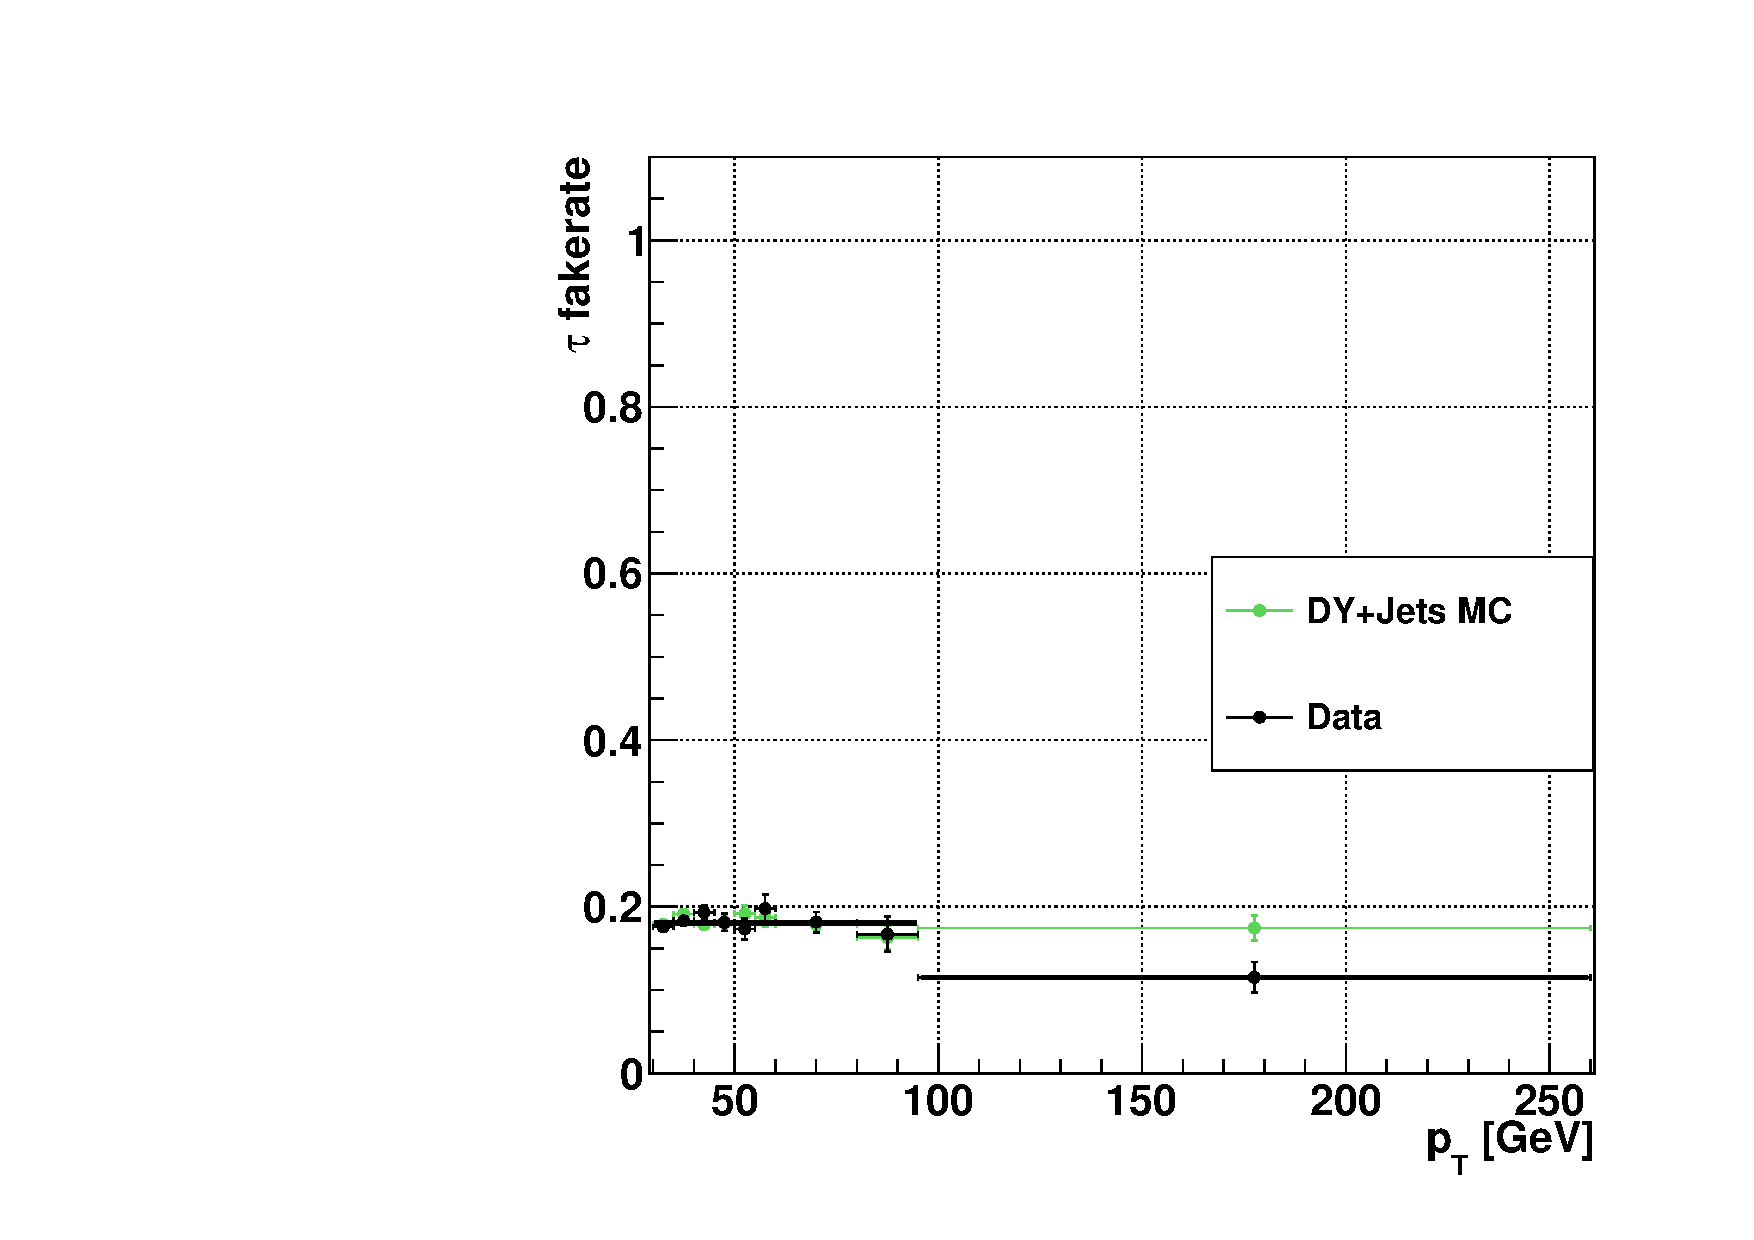
\includegraphics[width=0.3\textwidth]{chapterfakerate/preselectionDecay10_preselectionVLooseIsoDecay10_tPt_fakeRate.pdf}}\\
     \caption{$f_{\tau}$ ratio for the $\tau$ fake rate calculation shows in term of tau decay modes and $\pt$}
     \label{fig:fakerationumber}
\end{figure}

The misidentified muon events in the high mass LFV search are less than 5\% of the total misidentified events, so misidentified muon events are not considered. Study has been performed with Z+jets events, similar to the misidentified $\tau$ lepton study. As shown in Fig.~\ref{fig:MisidentifiedMuon}, in which the misidentified muons are added in and plotted separately with the misidentified $\tau$, compared with misidentified taus, misidentified muons are much less and  neglectable. 

\begin{figure}[htbp] 
\centering
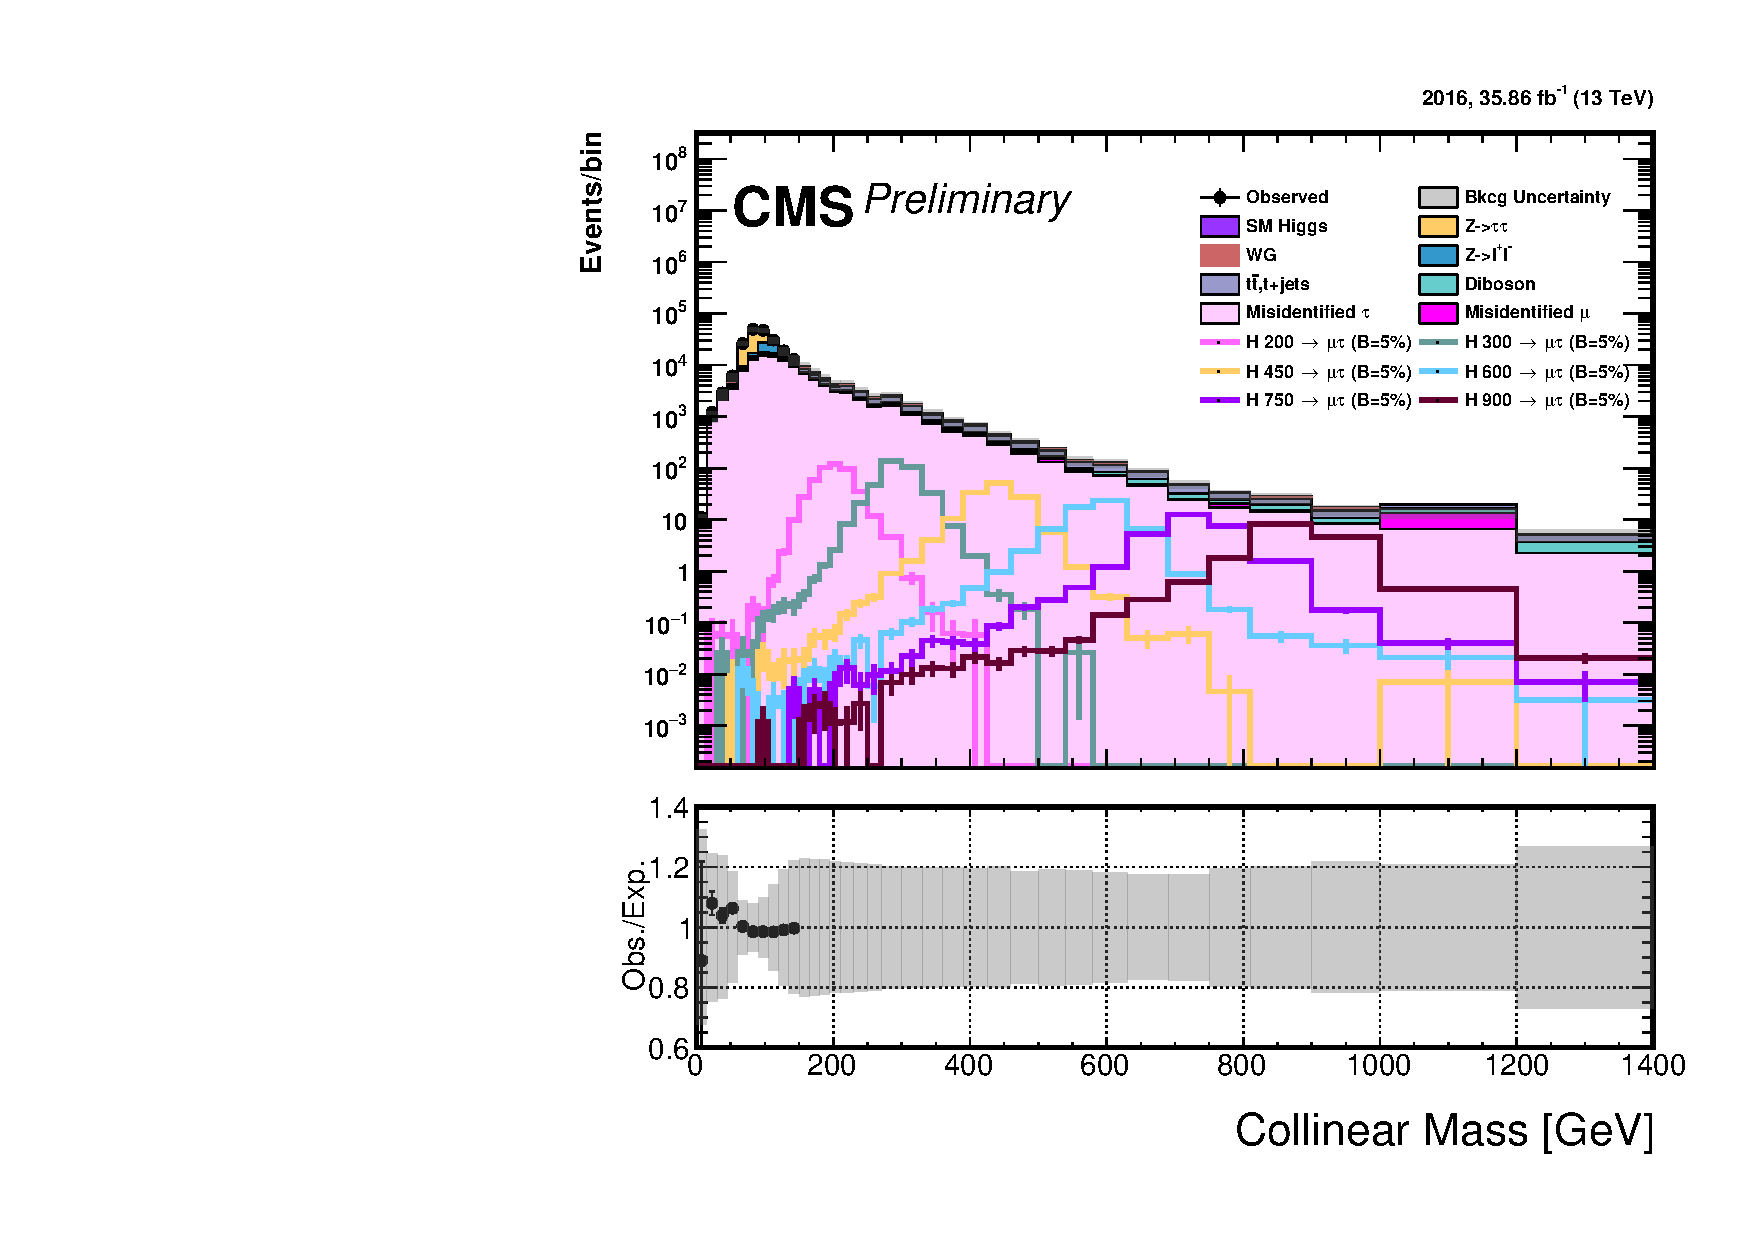
\includegraphics[width=0.6\textwidth]{chapterfakerate/LFV_preselection_collMass_type1_200Fakes_PoissonErrorsMuonfake.pdf}
\caption{Base selection $M_{col}$ distribution with misidentified muons added .}
\label{fig:MisidentifiedMuon}
\end{figure}

The validation of the misidentified lepton background with full data driven method is performed in a like-sign sample and W+jets enriched control region. In $\Hmuhad$ channel, the like-sign sample validation requires the events pass the loose selection, the same as the signal region, but with inverted charge. Misidentified background is enriched with the requirement of inverting charge. In the W+jets enriched control region, events that pass the loose selection are further selected with  $M_T(\tau)>60$ GeV and $M_T(\mu)>80$ GeV.  In both of the control regions, misidentified background is the dominant one, as shown in Fig.~\ref{fig:fakebackgroundValidation}. With full data driven method, applied with the $\tau(f_{\tau})$ as weight, the like-sign and W+jets control regions show good data and MC agreement. 


\begin{figure}[htbp] 
     \centering
     \subfigure[Wjets enriched control region]{ 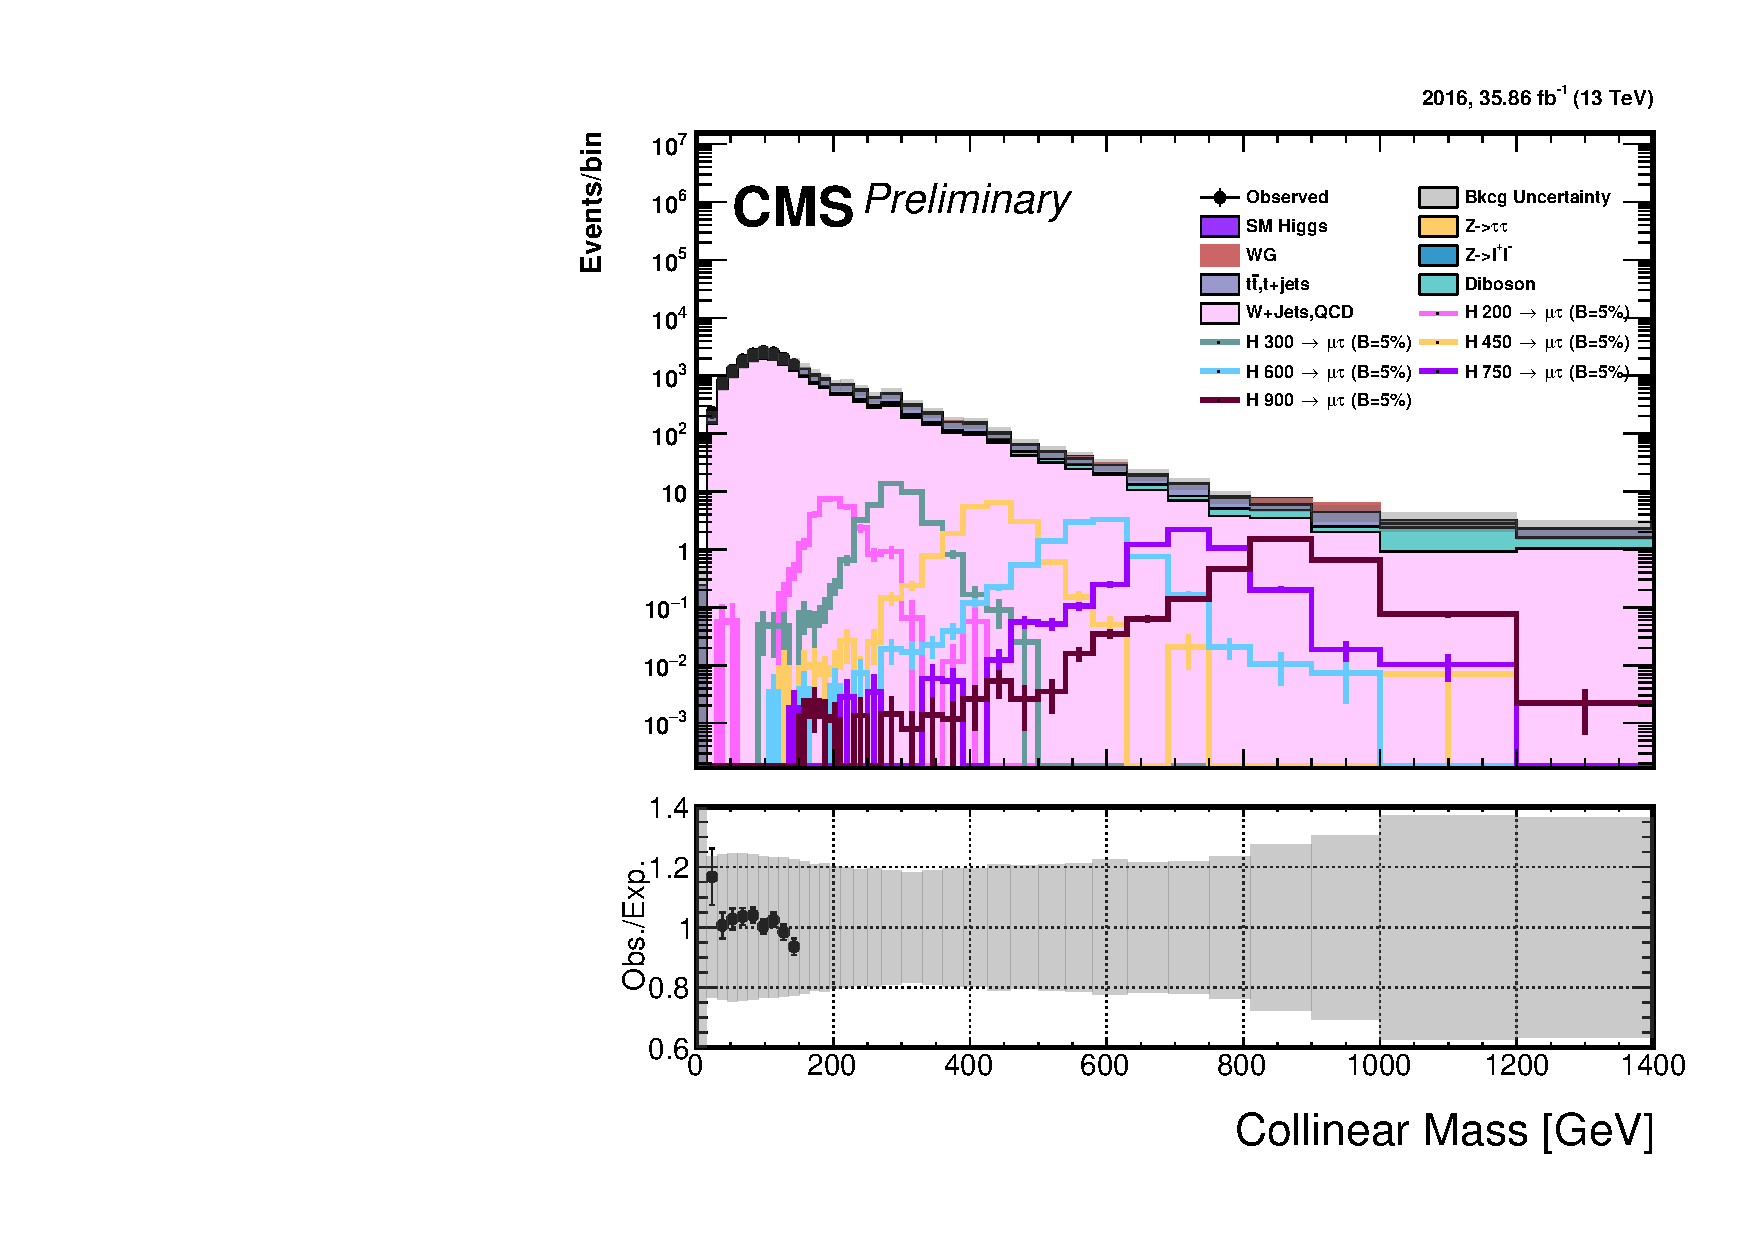
\includegraphics[width=0.4\textwidth]{chapterfakerate/LFV_preslectionEnWjets_collMass_type1_Fakes_PoissonErrors.pdf}}
     \subfigure[Like-sign control region]{ 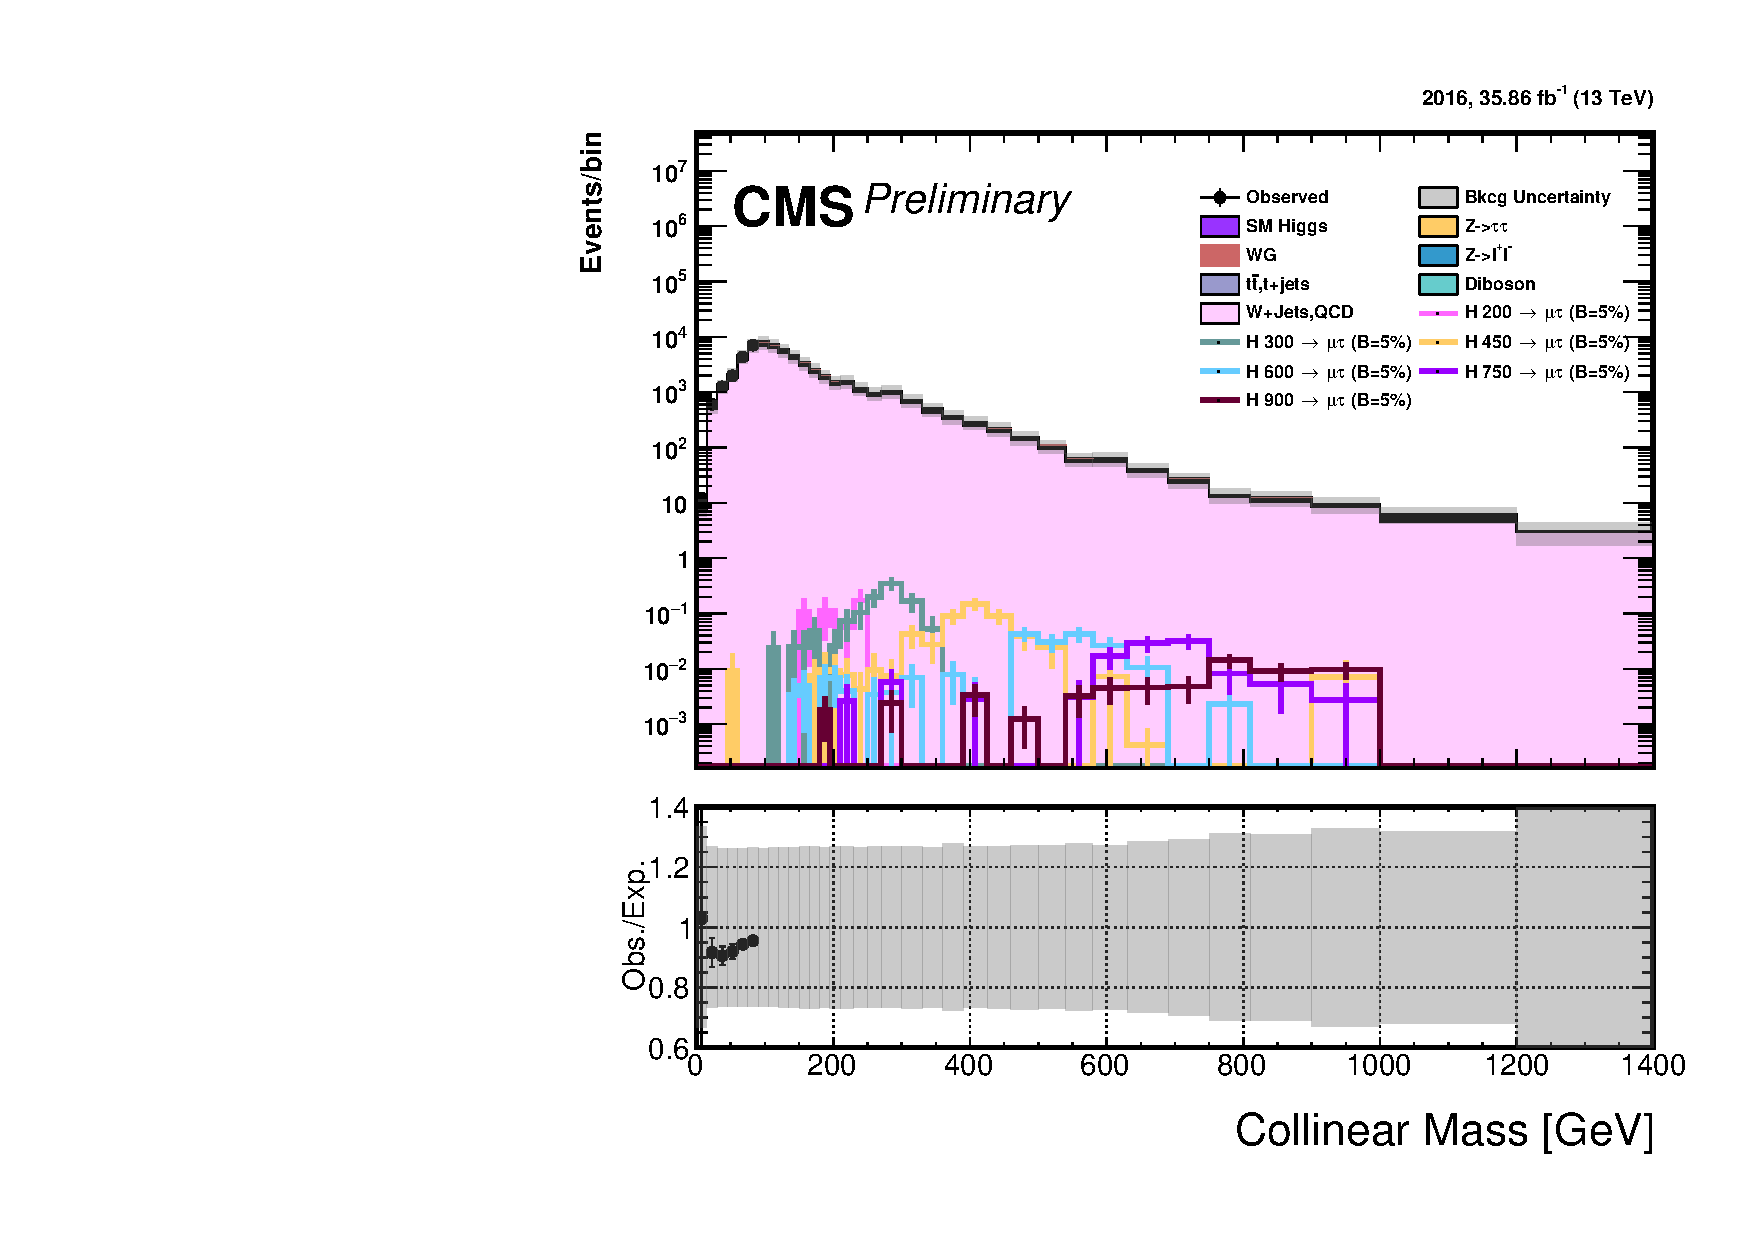
\includegraphics[width=0.4\textwidth]{chapterfakerate/LFV_preselectionSS_collMass_type1_Fakes_PoissonErrors.pdf}}
     \caption{The validation of full data driven method for the misidentified lepton background. 30\% of uncertainty is assumed in both cases. }
     \label{fig:fakebackgroundValidation}
\end{figure}









